\documentclass[12pt,a4paper]{article}
\usepackage{cmap}
\usepackage[T1, T2A]{fontenc}
\usepackage[utf8]{inputenc}
\usepackage[russian]{babel}
\usepackage{amsmath,amssymb}
\usepackage{parskip}
\usepackage{caption}
\usepackage{textcomp}
\usepackage{gensymb}
\usepackage[dvips]{graphicx}
\usepackage{wrapfig}
\usepackage{color}
\usepackage{setspace}
%\usepackage{hyperref}
\usepackage{epstopdf}

\oddsidemargin=-0.5 cm
\evensidemargin=-0.5 cm
\textwidth=170 mm
\textheight=260 mm
\topmargin=0 cm
\voffset= -2cm
\pagenumbering{false}
%\newlength{\varheight}
%\setlength{\varheight}{3.1cm}
\setlength{\parindent}{0cm}
\spacing{1.1}
\parskip=2mm
\clubpenalty=10000
\widowpenalty=10000

\begin{document}

\textit{``Из идей, в некотором роде, вариационного характера можно предположить, что кривая нити будет плавно изменяться по ходу изменения величины начиная с некоторого (критического) значения данной величины''}

Да, это похоже на правду. По крайней мере, моими численными расчетами подтверждается до 20-го знака.

\textit{``.. если мы теперь мысленно заменим нить вертикальным абсолютно твердым стержнем той же линейной плотности, ничего, в принципе, не измениться''}

А вот этот вывод неправильный. Легко понять, что оба момента линейны по углу отклонения, и следовательно их соотношение чувствительно к \textit{относительной} форме нити. То есть, если нить стремится к вертикальной прямой неравномерно вдоль длины, то ее нельзя заменять на прямую. Такая замена не изменит порядок величин моментов, однако может изменить соотношение между ними. Например, при ``спрямлении'' нити ее центр масс смещается, следовательно момент силы тяжести изменяется на коэффициент порядка единицы --- нарушая соотношение между моментами. Между тем, нам интересен случай, когда один момент (центробежный) начнет преобладать над другим, не по порядку, а с точностью до всех коэффициентов.

\begin{figure}[!h]
\begin{center}
 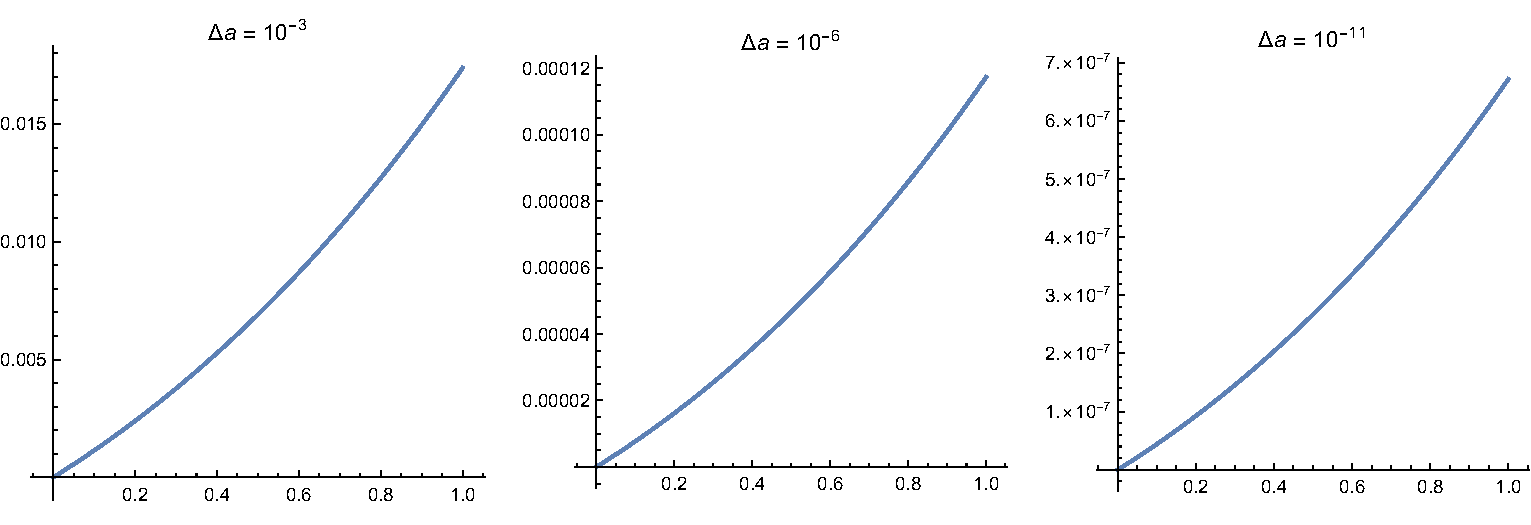
\includegraphics[width=\textwidth]{roperesp1.pdf}
\end{center}
\end{figure}

На графиках изображен профиль нити $x(y)$ при разных значениях разности величины $a$ и ее критического значения. Как видим, он стремится к некоторой функции, но никак не к прямой.

Можно обосновать это утверждение более строго. Если посмотреть на дифур при малых отклонениях от вертикали, можно получить
$$
  (1-\lambda)z''+az=0.
$$
Такой дифур, очевидно, не имеет линейного решения.

К сожалению, не все так просто :) Стоит сказать, что результат был близок к точному.

\end{document}

